\chapter{Range min-Max tree k-ária}
\label{chp:desenvolvimento}
Este capítulo refere-se ao objetivo central deste trabalho, apresentando a proposta de modificação da estrutura criada por \cite{paper-fully-functinal-succint-trees}. Mostraremos primeiro no que consiste essa adaptação, após isso apresentaremos a forma como a rmM-tree k-ária deve ser construída, apresentando também as operações suportadas por esta estrutura. 
Destaca-se também que os exemplos usados como base neste capítulo, são os mesmos exemplos usado no capítulo de apresentação da rmM-tree clássica, afim de facilitar a compreensão e comparação das duas propostas.

\section{Visão Geral}
Para este trabalho buscamos unir algumas características das árvores B com a range min-Max tree. Com até $k$ filhos, as árvores B possuem altura igual à $\log_k n$, e alto fator de ramificação, essas características combinadas a range min-Max tree, que é uma estrutura compacta, e portanto cabe na memória principal, possibilitará um uso otimizado de cache, como discutido no Capítulo~\ref{ch:fundamentacao}.

Dado uma representação em parênteses balanceados de uma árvore $T$, é escolhido um tamanho de bloco $b$. Esse tamanho de bloco, assim como na estrutura clássica define o tamanho de cobertura de cada intervalo compreendido por um registro.  Na proposta original \citet{paper-fully-functinal-succint-trees}, cada nó da range min-Max tree é responsável pela cobertura de um único intervalo, nesta adaptação propõe-se o agrupamento múltiplo de intervalos em nós.

Com base nisso, após definir uma aridade $k$, para a rmM-tree, seguindo a mesma abordagem \textit{bottom-up} da rmM-tree binária, construímos os nós folhas da nossa estrutura, armazenando até $k$ registros  \footnote{As árvores $B$, armazenam no máximo $k-1$ chaves por nó, em nossa estrutura limitamos o número de regitros de um nó à $k$.} (que cobrem intervalos de tamanho $b$) de valores de excesso por nó folha da nossa estrutura. Terminando de construir os nós folhas, iniciamos a construçãos dos nós internos da range min-Max tree k-ária, nível a nível, partindo do penúltimo nível da árvore. 

Cada nó $v$ (sendo $v$ não folha) da árvore será construído a partir da união de seus $k$ filhos, sendo que cada registro de um nó $v$ cobrirá o agrupamento dos registros do nó $k \cdot v +1 + i_{registro}$. 
Dessa maneira temos o exposto: se na versão clássica  da rmM-tree cada nó folha armazena no máximo um intervalo, e portanto possui $r=\ceil{n/b}$ folhas, 
na versão k-ária teremos $r=\ceil{n/(b \cdot k)}$ folhas. Como a altura de uma árvore pode ser calculada a partir de $h = \ceil{\log_k r}$ essa simples mudança reduzirá drasticamente a altura da nossa estrutura,
quando comparada a rmM-tree clássica,  potencialmente reduzindo o número de eventuais transferências de dados entre cache e RAM.

Tomemos como exemplo um tamanho de bloco $b = 32$, suponha um vetor que codifica um árvore $T$, de tamanho igual à  $4.675.776.358$, e que a nossa rmM-tree k-ária tem ordem igual à $16$. A tabela abaixo ajuda a esclarecer o exposto acima, mostrando a altura e a quantidade de folhas para cada versão da rmM-tree.


\begin{table}[h!]
    \centering
    \caption[Diferentes range min-Max tree sobree um conjunto de dados]{Altua e número de nós folhas para uma rmM-tree binária e k-ária}
    \label{tbl:dataset}
      \resizebox{\columnwidth}{!}{
          \begin{tabular}{|l|l|l|l|l|}
          \hline
          \textbf{Tipo}                       & \textbf{Tamanho da árvore de entrada}                     & \textbf{Quantidade de folhas da rmM-tree}                       & \textbf{Altura da rmM-tree}     \\ \hline
          binária                             & $4.675.776.358$       & $\ceil{4.675.776.358/32} = 146.118.012$     & $\ceil{\log_2(146.118.012)} = 28$    \\ \hline
        16-ária                             & $4.675.776.358$       & $\ceil{(4.675.776.358/(32 \cdot 16))} =  9.132.376$ & $\ceil{\log_{16}(4.711.244)} =  6$ \\ \hline 
          \end{tabular}
      }
  \end{table}

 Ao aumentarmos o fator de ramificação de uma árvore, tiramos proveito do princípio de localidade espacial, que afirma que itens cujos endereços estão próximos um do outro tendem a ser referenciados em um curto espaço de tempo \citep{book-computer-architecutre}, diminuindo assim o número de eventuais transferência de dados entre cache e memória RAM.
 
%pg 524
\section{Registros}
Os registros da range min-Max tree k-ária permanecem exatamente os mesmos, sendo eles: \textit{excesso local (e)}, que indica o excesso total  computado em um intervalo; \textit{excesso local mínimo (m)} que é relativo ao menor excesso computado em um intervalo $[s,e]$; \textit{excesso local máximo (M)} que é análogo ao excesso mínimo; e \textit{número de vezes que o excesso mínimo ocorre (n)} em um intervalo. A grande diferença, é que agora esses valores de excessos estão agrupados em até $k$ blocos de tamanho $b$ por folha, isso nos dá às seguintes relações para os nós internos e raíz:

\begin{itemize}
    \item $R[v][rg].e = \displaystyle{\sum_{i=0}^{l-1} R[j][i].e} $
    \item $R[v][rg].m = min(R[j][0].m, ... , R[j][0].e + ... + R[j][l-1].e + R[j][l].m )$
    \item $R[v][rg].M = Max(R[j][0].M, ... , R[j][0].e + ... + R[j][l-1].e + R[j][l].M )$
    \item $R[v][rg].n =$ número de vezes que o excesso mínimo computado aparece nos registros de  $j$.  
\end{itemize}

em que:
\begin{itemize}
    \item $rg$, é o $rg-$ésimo registro de $v$ e aponta para o nó $j =(v\cdot k)+1+rg$ (com $0 \leq rg <  k$ );
    \item $j$ é o $j-$ésimo filho de $v$;
    \item $l$ é a quantidade de registros em $j$.
\end{itemize}


\begin{example}
    Usando o Exemplo~\ref{ex-build-tree} de sequência de parênteses balanceados da Seção~\ref{sec:sec-classic-rmm-tree}, assuma uma cobertura de bloco igual à $4$, e uma rmM-tree de  ordem também igual à $4$.  Com base nas definições anteriores, temos que a range min-Max tree terá $4$ nós folhas, e no máximo $4$ registros por nó, pois:

    $$r = \ceil{n/(b \cdot k)} \to \ceil{(52/16)} = 4$$
    $$h = \ceil{\log_k r} \to \ceil{\log_4 4} = 1 $$
        
        Iniciamos a construção da nossa árvore partindo dos nós folhas, como estamos utilizando o mesmo exemplo da Seção~\ref{sec:sec-classic-rmm-tree}, cada uma de nossas folhas será idêntica ao agrupamento de $4$ folhas consecutivas do Exemplo~\ref{ex-build-tree} (a nossa folha $0$ corresponde ao agrupamento das folhas $0,1,2 \mbox{ e } 3$ da estrutura binária, por exemplo). A altura da range min-Max tree k-ária, neste exemplo é $1$, e portanto temos apenas o nó raíz acima das nossas folhas. Cada registro do nosso nó raíz, cobrirá a união dos registros dos seguintes nós\footnote{R[i][j] = R[nó][registro]}:
        \begin{itemize}
            \item $R[0][0]$ cobre a união dos registros do nó $1$, pois: $(0 \cdot 4) +1 + 0=1 \therefore$ \\
            $R[0][0].e = R[1][0].e + R[1][1].e R[1][2].e + R[1][3].e = 2$;\\
            $R[0][0].M = 4$, pois:\\
            \begin{eqnarray*}
                \begin{split}
                    R[0][0].M =& max(R[1][0].M, \\
                    &   R[1][0].e + R[1][1].M, \\
                    &   R[1][0].e + R[1][1].e + R[1][2].M,  \\
                    &   R[1][0].e + R[1][1].e + R[1][2].e + R[1][3].M)\\
                    &   = max(4,4,4,4) = 4;
                \end{split}
            \end{eqnarray*}
            $R[0][0].m = 1$, pois:
                \begin{eqnarray*}
                    \begin{split}
                        R[0][0].m =& min(R[1][0].m, \\
                        &   R[1][0].e + R[1][1].m, \\
                        &   R[1][0].e + R[1][1].e + R[1][2].m,  \\
                        &   R[1][0].e + R[1][1].e + R[1][2].e + R[1][3].m)\\
                        &   = min(1,3,2,2) = 1;
                    \end{split}
                \end{eqnarray*}
                $R[0][0].n = 1$.
            \item $R[0][1]$ cobre os registros do nó $2$, pois: $(0 \cdot 4) +1 + 1=2$, e
            $$R[0][1].e = 0; R[0][1].M = 2; R[0][1].m=-1 \mbox{e } R[0][1].n=2.$$
            \item $R[0][2]$ compreende a união dos registros do nó $3$, pois: $(0 \cdot 4) +1 + 2=3$, e
            $$R[0][2].e = 0; R[0][2].M = 1; R[0][1].m=-1 \mbox{e } R[0][1].n=1.$$
            \item $R[0][3]$ cobre a união dos registros do nó $4$, pois: $(0 \cdot 4) +1 + 2=4$, e
            $$R[0][3].e = -2; R[0][3].M = 1; R[0][1].m=-2 \mbox{e } R[0][1].n=1.$$
        \end{itemize} 

        Observe que, se unirmos os intervalos que compõem os registros do nó $0$, obteremos um registro equivalente ao do nó raíz mostrado no exemplo da construção da rmM-tree binária.
\end{example}

O processo de construção da rmM-tree k-ária é similar ao processo de construção da rmM-tree binária, descrito no Capítulo~\ref{ch:fundamentacao}, a diferença é que, para este caso precisaremos guardar em um nó até $k$ registros de excesso. Podemos para tanto fazer o uso de uma estrutura auxiliar como uma lista ou um vetor (presente em linguagens de programação como C++), onde cada elemento dessa estrutura representará os registros, de um nó $v$ da rmM-tree, ao qual essa estrutura auxiliar está associada. A \figref{fig:rmm-tree-k} mostra a representação gráfica da range min-Max treee k-ária usada no exemplo acima.


\begin{figure}[h!]
    \centering
      \caption[rmM-tree 4-ária.]{rmM-tree 4-ária, com tamanho de bloco igual à 4. No canto superior esquerdo de cada nó, em negrito,
        é mostrado o índice do mesmo na rmM-tree, já no canto inferior esquerdo de cada folha, em azul, vemos a ordem da mesma.}
      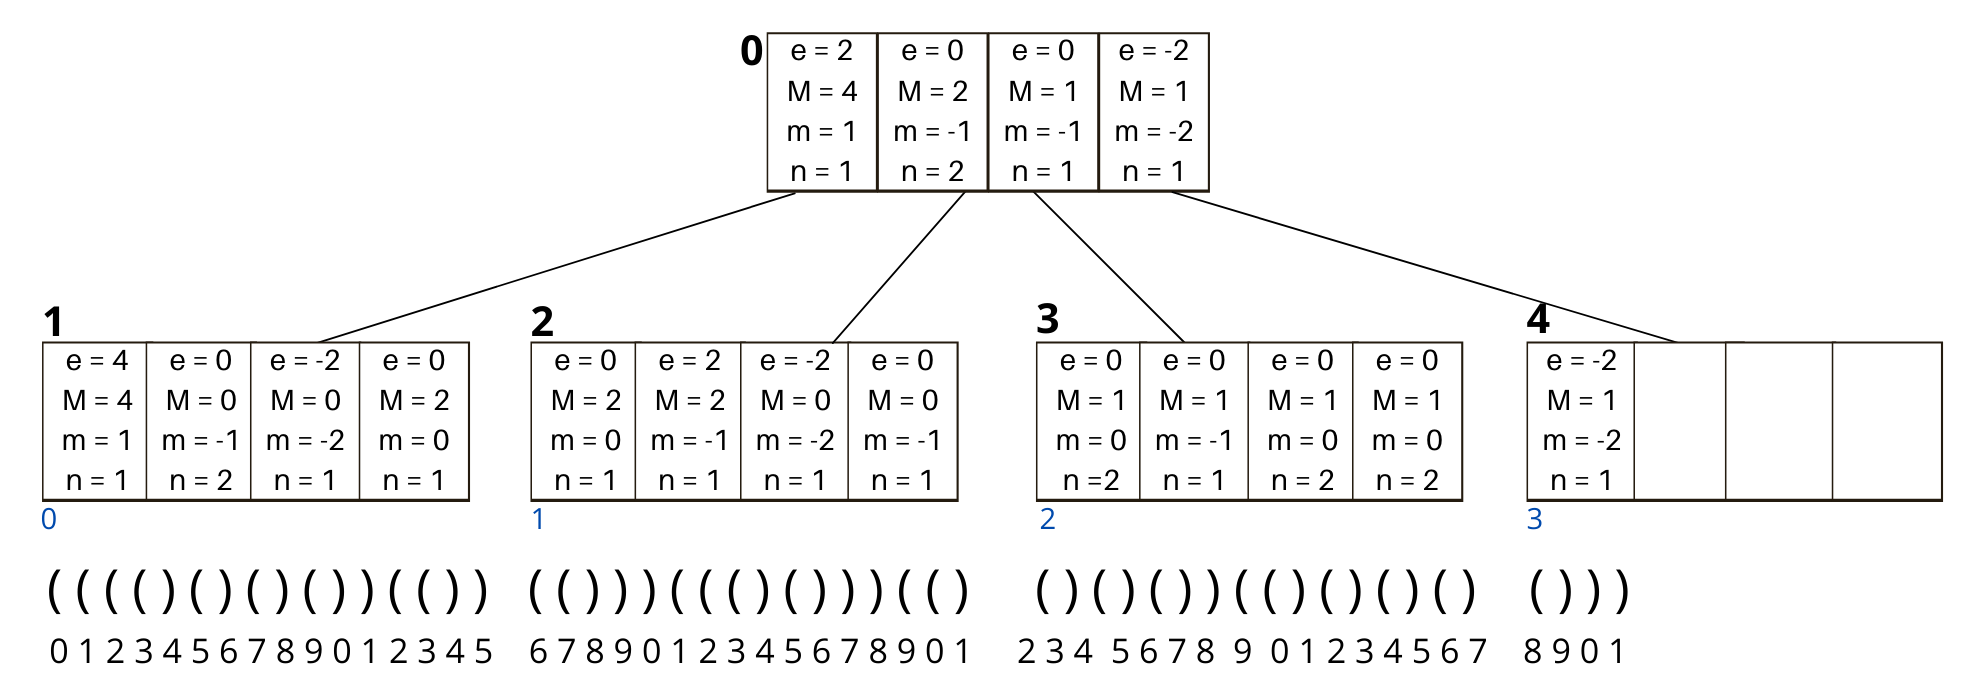
\includegraphics[width=\columnwidth]{images/rmm-tree-kary.png}
      \label{fig:rmm-tree-k}
    \end{figure}

    \begin{algorithm}[h!]
        \SetKwFunction{algo}{algo}
        \SetKwProg{myalg}{Algoritmo}{}{}
        \myalg{buildingTree(BP, C, k, b, w, r, nNodes)}{
    
            \Input{Vetor de bits, tabela de excessos C, aridade da árvore, tamanho de bloco e de subbloco, número de folhas e quantidade de nós.}
    
            \tcp{Construção dos nós folhas}
            $numReg \leftarrow 0$\\
            \For{$l \leftarrow 0$ \textbf{to} $r -1$}{
                $v \leftarrow leafInTree(l)$\tcp{Análogo ao Algoritmo~\ref{alg:folha-indice}}
                $reg \leftarrow 0$\\
                \While{$R[v].nReg < k$ \textbf{and} $numReg < \ceil{BP.size()/b}$}{
                    $(R[v][reg], R[v][reg].M, R[v][reg].m, R[v][reg].n) \gets(0,-w,w,0)$\\
                    \For{$p \leftarrow (numReg\cdot (b/w))+1$ \textbf{to} $((numReg+1)\cdot b)/w$}{
                        $x \leftarrow bistread((p-1)\cdot w)$\\
                        \lIf{$R[v][reg].e + C[x].M > R[v][reg].M$}{$R[v][reg].M \leftarrow R[v][reg].e + C[x].M $}
                        \lIf{$R[v][reg].e + C[x].m < R[v][reg].m$}{$R[v][reg].m \leftarrow R[v][reg].e + C[x].m $}
                        \ElseIf{$R[v][reg].e + C[x].m = R[v][reg].m$}{$R[v][reg].n \leftarrow R[v][reg].n + C[x].n$}
                        $R[v][reg].e \leftarrow R[v][reg].e + C[x].e$
                    }
                    $R[v].nReg \leftarrow R[v].nReg  +1$\\
                    $numReg \leftarrow numReg +1$\\
                    $reg \leftarrow reg +1$
    
                } 
            }
            \tcp{Construção dos nós internos e raíz}
            \For{$v \leftarrow nNodes - r - 1 $ \textbf{to} $0$}{
                \For{$reg \leftarrow 0$ \textbf{to} $k-1$ \textbf{and} $(v\cdot k)+reg+1$ \textbf{to} $nNodes-1$}{
                    $child \leftarrow (k\cdot v)+1+reg$\\
                    $R[v][reg].e  \leftarrow R[child][0].e$\\
                    $R[v][reg].m \leftarrow R[child][0].m$\\
                    $R[v][reg].M \leftarrow R[child][0].M$\\
                    $R[v][reg].n \leftarrow R[child][0].n)$\\
    
                    \For{$i \leftarrow 1$ \textbf{to} $R[child].nReg-1$}{
                        $R[v][reg].M = max(R[child][i-1].M,R[v][i-1].e + R[child][i].M) $\\
                        $R[v][reg].m = min(R[child][i-1].m,R[v][i-1].e + R[child][i].m) $\\
                        \If{$R[v][reg].m < R[child][i-1].e + R[child][i].m$}{
                            $R[v][reg].n \leftarrow R[child][i].n$
                        }
                        \ElseIf{$R[v][reg].m = R[child][i-1].e + R[child][i].m$}{
                            $R[v][reg].n \leftarrow R[v][reg].n  + R[child][i].n$
                        }
                        $R[v][reg].e \leftarrow R[child][i].e$\\
                    }
                }
    
            }
        } 
        \caption{Construção da range min-Max tree k-ária}
        \label{alg:build-kary-rmm-tree}
    \end{algorithm} 

O Algoritmo~\ref{alg:build-kary-rmm-tree} ilustra o processo de construção da rmM-tree k-ária. A tabela C, as funções \textit{bitsread, leafInTree} e \textit{numLeaf} -- algumas citadas nesse e em outros algoritmos -- seguem a mesma abordagem da rmM-tree clássica. O elemento \textit{nReg} associado à um nó $v$ corresponde, ao número de registros naquele nó.



\section{Operações}\label{sec:optimized-operation}
Para este trabalho a nossa estrutura fornece suporte às duas principais primitivas da Range min-Max tree clássica, fwdSearch e bwdSearch (além daquelas já suportadas pela estrutura de vetores de bits). Além destas duas, nossa árvore de intervalos máximos e mínimos, fornece suporte à 5 operações derivadas daquelas apoiadas pela estrutura de vetores de bits (sobre a qual a nossa árvore é construída), e outras 16 operações, que são derivadas das duas primitivas exploradas adiante.


\subsection{FwdSearch}\label{sec:fwdSearch}
Como já dito no capítulo anterior a operação foward search, realiza uma busca a partir de um índice \textit{i}, afim de encontrar a posição $j>i$, onde ocorre um excesso relativo \textit{d}.

Essa operação, nessa versão da rmM-tree, se dá parcialmente de igual forma ao do modo clássico: varremos primeiro o bloco da folha, em busca do excesso desejado, a partir de $i+1$.  A diferença é que agora precisamos verificar  até \textit{k} blocos de tamanho \textit{b} dentro de cada nó inspecionado na nossa estrutura. Para tanto, acrescentamos à fwdSearch em sua versão clássica duas outras funções, são elas fwdRegistry e fwdVerifySibling.

A primeira função é chamada sempre que estamos visitando um nó folha, ou seja no início da busca e ao final da mesma, quando já encontramos o nó alvo que contém a resposta.  A operação fwdRegistry tem por objetivo identificar o registro que contém o excesso buscado da folha analisada. O processo é muito similar à verificação de um nó na rmM-tree clássica: a cada registro pecorrido verificamos a asserção $dr + R[v][reg].m \leq d \leq dr + R[v][reg].M$, caso seja verdadeira, significa que encontramos o intervalo que contém a resposta desejada. Se a asserção for falsa, adicionamos ao excesso relativo computado até o momento ($dr$), o excesso local do registro que acabamos de visitar, seguindo para o próximo registro.  O Algoritmo \ref{alg:fwdRegistry} fornece mais detalhes de como esse processo de busca por excesso nas folhas funciona.

Caso o excesso buscado não seja encontrado na folha inicial, acionamos o processo de subida na árvore, aliado à nova função que mencionamos, \textit{fwdVerifySibling}. O objetivo dessa função é similar ao proposto por \citet{book-compact-data-structures}, quando o autor sugere que em cada nível verifiquemos se o excesso procurado está no irmão à direita do nó atual. Assim \textit{fwdVerifySibling} calcula a quantidade de irmãos do nó $v$ existentes à sua direita, e então analisa os registros de cada um deles em busca do intervalo que contém o excesso buscado, atualizando o valor de $dr$ sempre que $d$ não for encontrado em um registro.

Se ao final da inspeção dos irmãos de $v$, não encontrarmos o registro que contém a resposta, atualizamos o valor de $v$ para o índice do seu nó pai, e verificamos os irmãos deste nó atualizado. Repetimos esse processo até que seja encontrado um registro que contenha o excesso relativo desejado.

Tendo encontrado o intervalo que contém a resposta desejada durante a subida na rmM-tree, iniciamos  o processo de estreitamento desse intervalo, através do processo de descida na rmM-tree. Esta etapa é  similar as demais, e consiste em pecorrer os registros de um nó $v$, verificando se a asserção $dr + R[v][reg].m \leq d \leq dr + R[v][reg].M$ é válida, atualizando o valor do excesso computado até o momento, sempre que necessário. Ao inspecionarmos um registro que contém a resposta buscada,  atualizamos o valor de $v$, com base nesse registro, descendo mais um nível da árvore. Repetimos esse processo até que cheguemos à um nó folha, que é quando executamos novamente \textit{fwdRegistry}.

Os Algoritmos \ref{alg:fwdVerifySibling} e \ref{alg:fwdSearch} mostram como o processo de descida na árvore funciona, bem como o funcionamento completo de \textit{fwdSearch}.



O exemplo a seguir é baseado no Exemplo~\ref{ex:bin-fwdSearch} da Seção~\ref{sec:fwdsearch-bin}, e demonstra como podemos usar a operação \textit{fwdSearch} para obtermos a demarcação de término de um nó.
\begin{example}
Dado um nó em $BP$, codificado em $i=21$, encontrar o primeiro índice $j>i$, tal que $excess(j) - excess(i) = -1$.

O processo para a obtenção dessa resposta é descrito a seguir:

 O primeiro passo é identificar  o índice e o registro do nó folha que cobre $i=21+1$ (lembrando que a busca é por um $j > i$), neste caso temos $v = 2$ (folha $1$), e $reg = 1$, pois $\floor{(21 - 16)/4} = 1$. Assim iniciamos a varredura, pecorrendo o nó $v$, a partir de $i+1$ até o final do registro $1$. Ao finalizar a inspeção do registro que contém $i$, 
 temos que o excesso computado até o momento ($dr$) vale $2$, e portanto não encontramos o excesso buscado.
 
 \begin{figure}[h!]
    \centering
      \caption[fwdSearch(21,-1).]{Simulação da operação \textit{fwdSearch(21,-1)}.}
      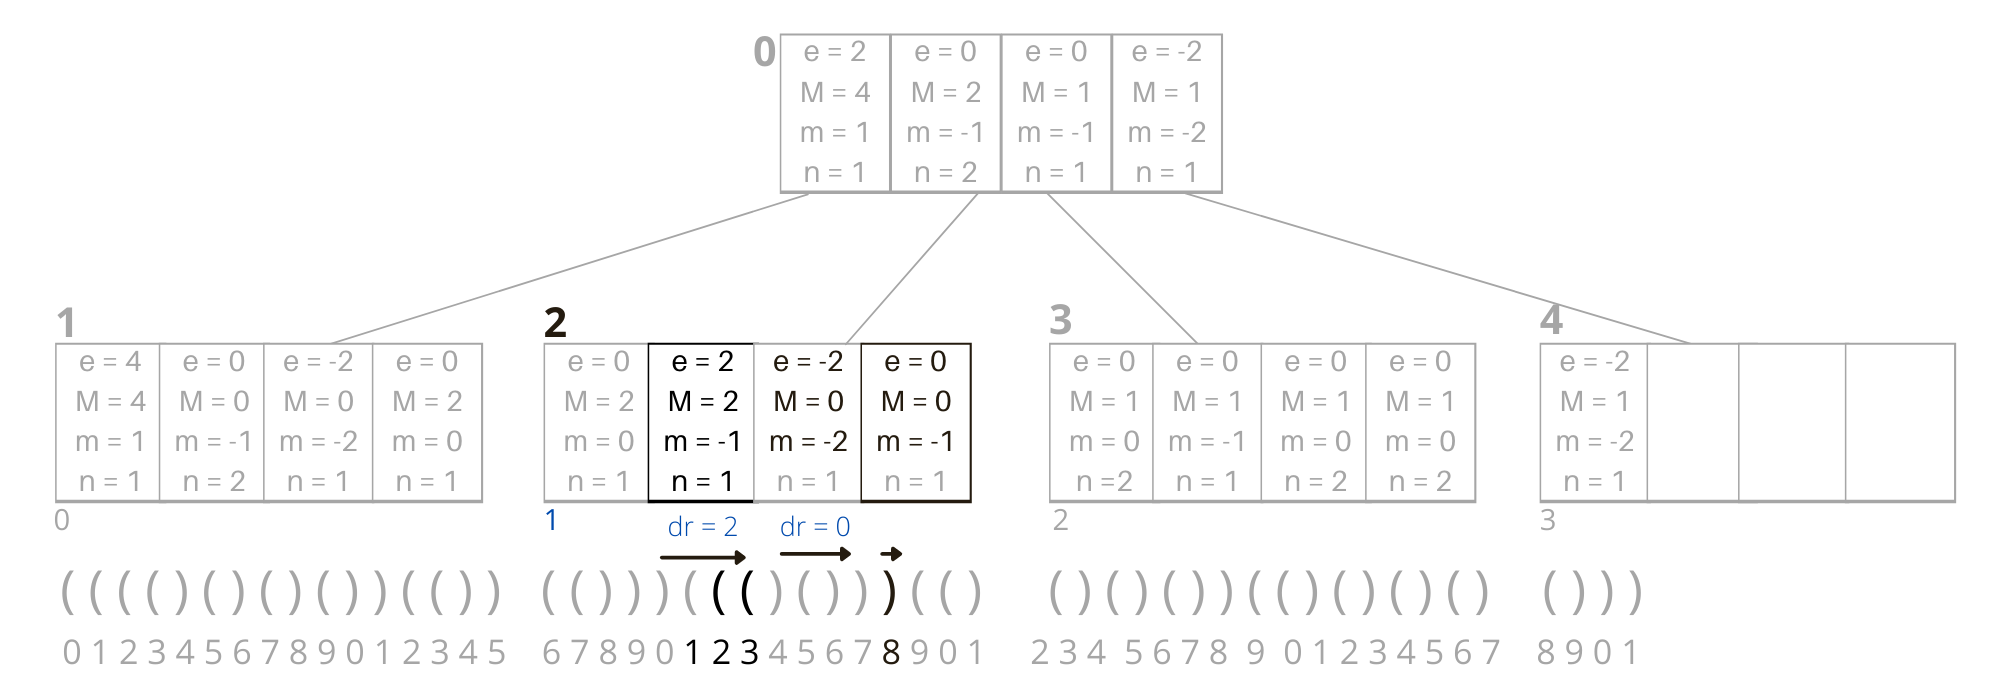
\includegraphics[width=\columnwidth]{images/rmm-tree-kary-fwdsearch.png}
      \label{fig:kary-fwdSearch}
 \end{figure}
\end{example}
Antes de verificarmos os irmãos do nó $v$, inspecionamos os registros restantes em $v$, analisando a cada momento se $dr + R[2][reg].m \leq d \leq dr + R[2][reg].M$. Ao verificar o registro $2$ do nó $v$, não encontramos o excesso buscado, atualizamos então o valor de $dr$, somando à ele $R[2][2].e$. Inspecionamos o último registro do nó $v=2$, e identificamos que $d$ está compreendido em seu intervalo. Interrompemos a análise dos nós da rmM-tree, e iniciamos uma análise mais detalhada da chave $3$, a fim de encontrar a posição exata onde $d$ ocorre. Durante essa inspeção, o valor de $dr$ atinge a marca $-1$, no índice $j=28$, encerrando assim a busca pelo excesso $d$ através de \textit{fwdSearch}.

 Perceba que neste exemplo foi necessário a inspeção de $2$ registros (excluindo o nó inicial), sem a necessida de realizar um percurso de subida na rmM-tree, ao passo que para o mesmo exemplo, na estrutura binária é necessário a inspeção de $5$ nós (excluindo o nó inicial), subir um nível, e depois descer um nível.

 \begin{algorithm}[htp]

    \SetKwFunction{algo}{algo}
    \SetKwProg{myalg}{Algoritmo}{}{}
    \myalg{fwdRegistry(i,v,reg,l,d,\&dr)}{
        \Input{Índice em $BP$, nó $v$, folha e registro correspondente, a partir dos quais a busca deve ser feita,  excesso relativo buscado, e excesso relativo computado em cada registro inspecionado ($d$ e $\&dr$). }
        \Output{Posição $j$ ou $BP.size()$ caso $d$ não seja encontrado.}
        \vspace{.3cm}
            \For{$reg$ \textbf{to}  $R[v].nReg -1$}{
                \If{$(dr + R[v][reg].m  \leq  d \leq  dr + R[v][reg].M)$}{
                    $j \leftarrow fwdBlock(i,d,dr)$\tcp{Algoritmo~\ref{alg:fwdBlock}}
                    \If{$dr = d$}{ \Return{$j$ }}

                }
                $dr \leftarrow dr +  R[v][reg].e$\\ 
                $i \leftarrow (k\cdot l+reg+1)\cdot b -1$ \tcp{calcula o fim da registro atual}
                \If{$dr = d$}{\Return{$i$ }}
            }
            \Return{$BP.size()$}
    }
    \caption{Verificando os registros de um nó folha.}
    \label{alg:fwdRegistry}
    \end{algorithm}
    
\begin{algorithm}[htp]
        \SetKwFunction{algo}{algo}
        \SetKwProg{myalg}{Algoritmo}{}{}
        \myalg{fwdVerifySibling(\&v,\&dr,d)}{
            \Input{Nó $v$,  excesso relativo buscado e excesso relativo computado até o momento e excesso buscado. }
            \Output{Registro $(reg)$ que contém a resposta, ou $BP.size()$ caso o intervalo que contém $d$ não seja encontrado.}
            \vspace{.3cm}
            $parent \leftarrow \floor{(v-1)/k}$ \\
            $n\_sibling \leftarrow v - (parent \cdot  k)$\\
            $v \leftarrow v + 1$\\
            \While{$n\_sibling$ \textbf{to}  $R[parent].nReg -1$ \textbf{and} $v$ \textbf{to} $num\_nodes - 1$}{
                \For{$reg \leftarrow 0$ \textbf{to} $R[v].nReg -1$}{
                    \If{($dr + R[v][reg].m  \leq  d \leq  dr + R[v][reg].M)$}{
                        \If{$v \leq numberNodes - numberLeaves$}{$v \leftarrow (v\cdot k)+1+reg$}
                        \Return{$reg$ }
                    }
                    $dr \leftarrow dr +  R[v][reg].e$\\
                    \If{$dr = d$}{
                        \If{$v \leq numberNodes - numberLeaves$}{$v \leftarrow (v\cdot k)+reg+2$}
                        \Return{$reg+1$ }
                    }
                }
                $n\_sibling \leftarrow n\_sibling + 1$\\
                $v \leftarrow v+1$\\
                %TODO preciso ser tão precisa?exibir todas as condições do meu código?Lembrando que estou trabalhando com referencia 
            }
            \Return{$BP.size()$ }
        }
        \caption{Busca o excesso relativo nos irmãos à direita de $v$.}
        \label{alg:fwdVerifySibling}
    \end{algorithm}

\begin{algorithm}[htp]
    \SetKwFunction{algo}{algo}
    \SetKwProg{myalg}{Algoritmo}{}{}
    \myalg{fwdSearch(i,d)}{
        \Input{Índice a partir do qual a busca deve ser feita, excesso relativo buscado.}
        \Output{Posição $j$ onde ocorre o excesso $d$ ou $BP.size()$ caso $d$ não exista no intervalo definido.}
        \vspace{.3cm}
        $dr \leftarrow 0$\\
        $l \leftarrow \floor{(i+1)/(b\cdot k)}$\\
        $v \leftarrow leafInTree(l)$\\
        $reg \leftarrow \floor{( (i+1) - (l\cdot b\cdot k))/b}$\\
        $j \leftarrow fwdBlock(i,d,dr)$\tcp{Algoritmo~\ref{alg:fwdBlock}}

        \If{$dr = d $}{\Return{$j$}}

        $reg \leftarrow reg +1$\\
        \If{$reg < R[v].nReg$}{
            $j \leftarrow fwdRegistry((k\cdot l+reg)\cdot b-1,v,reg,l,d,dr)$\\
            \lIf{$dr = d $}{\Return{$j$}}
        }
        \vspace{.3cm}
       \tcp{Inicia o processo de subida na rmM-tree}
        \While{$v \neq 0$ \textbf{and} $fwdVerifySibling(v,dr,d) = BP.size()$ }{
            $v \leftarrow \floor{(v-1)/m}$\\
        }
        
        \tcp{Chegamos ao nó raíz, e $d$ não está em nenhum dos seus filhos}
        \If{$v=0$ \textbf{and} $reg=v.size()$}{\Return{$v.size()$}}
        \vspace{.3cm}
        \tcp{Inicia descida em árvore}
        \While{$v \leq numberNodes - numberLeaves$}{
            \For{$reg \leftarrow 0$ \textbf{to} $R[v].nReg -1$}{
                \If{$(dr + R[v][reg].m  \leq  d \leq  dr + R[v][reg].M)$}{
                    $v \leftarrow (v\cdot k) + 1 + reg $\\
                    $reg \leftarrow 0 $\\
                    \textbf{break}
                }
                \lElse{
                    $dr \leftarrow dr +  R[v][reg].e$
                }

            }
        }
        $l \leftarrow numLeaf(v)$\\
        $i \leftarrow (k\cdot l\cdot chave)\cdot sizeBlock$  \tcp{Calcula o índice inicial da folha que queremos inspecionar}
        $j \leftarrow fwdRegistry(i-1,v,0,l,d,dr)$\\
        \lIf{$dr = d$}{ \Return{$j$}}
        \Return{$BP.size()$}
    }
    \caption{Busca por um excesso relativo $d$, para um $j>i$}
    \label{alg:fwdSearch}
    \end{algorithm}

\newpage
         
\subsection{BwdSearch}\label{sec:bwdSearch}
Como dito anteriormente, o processo para calcular bwdSearch é completamente análogo à fwdSearch, devendo termos cuidado apenas com as questões relacionadas à simetria dos dados abordadas no Capítulo~\ref{ch:fundamentacao}. Tendo isso em mente podemos construir uma função que verifica se o excesso buscado está entre os registros das folhas analisadas, assim como uma segunda função que inspeciona os registros dos $p$ irmãos de um nó $v$. Os Algoritmos \ref{alg:bwdRegistry}, \ref{alg:bwdVerifySibling} e \ref{alg:bwdSearch} mostram o pseudocódigo para as adaptações da estrutura k-ária.

%TODO colocar referência interna
Apenas para recapitularmos, temos as seguintes observações em relação à assimetria dos dados em  bwdSearch\footnote{Para mais detalhes, verifique a Seção~\ref{sc:bwdsearch}}:
\begin{itemize}
    \item A posição $i$ é incluída na contagem de excessos;
    \item Adicionamos $1$ ao excesso relativo computado a cada inspeção, quando passamos por um bit $0$, e subtraímos $1$ desse excesso quando varremos um bit codificado como $1$;
    \item $excess(i) + d $ é alcançado quando $dr - R[v][reg].e + R[v][reg].m \leq d \leq dr - R[v][reg].e + R[v][reg].M $ for verdadeiro.
\end{itemize}

O Exemplo~\ref{ex:kary-bwd}  demonstra como podemos realizar a busca por um parênteses de abertura que codifica um nó, dado o seu respectivo parênteses de fechamento, através da operação \textit{bwdSearch}. Este exemplo por sua vez, é equivalente ao Exemplo~\ref{ex:bin-bwd}.

\begin{example}\label{ex:kary-bwd}
    Dado um nó em $BP$, codificado em $i=50$, encontrar o  índice $j<i$ mais à direita de $i$,tal que $excess(j) - excess(i) = 0$.
    \begin{figure}[htp]
        \centering
          \caption[bwdSearch(50,0).]{Simulação da operação \textit{bwdSearch(50,0)}.}
          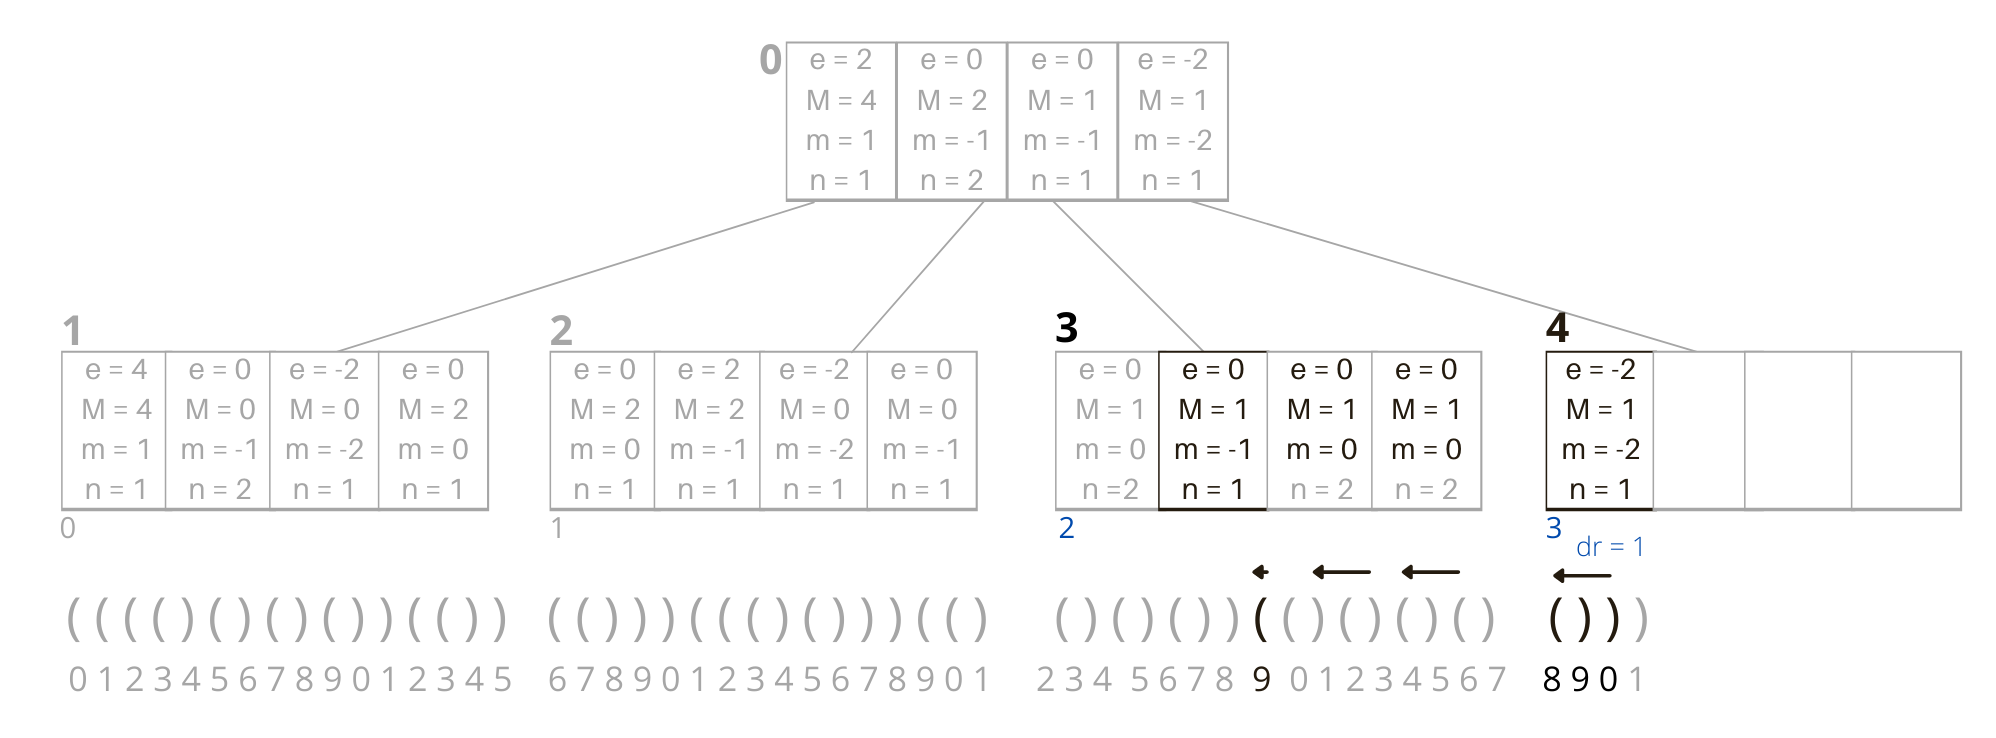
\includegraphics[width=\columnwidth]{images/rmm-tree-kary-bwdsearch.png}
          \label{fig:kary-bwdSearch}
     \end{figure}


     Após identificarmos o nó e o registro a qual pertence o índice $i=50$, temos que $v=4$ (folha $3$) e $reg = 0$ ($\floor{(50-48)/4}$). Iniciamos a inspeção da folha  $3$, partindo de  $i=50$, até alcançarmos o início da mesma que é $s=48$, ao término desta inspeção temos que $dr=1$. Como o nó $4$ não possui outros registros e a resposta não foi encontrada, realizamos a verificação dos registros localizados nos irmãos à esquerda do nó $v$.

     Atualizamos $v$ para o seu antecessor, que passa a valer $3$, pecorremos então cada um dos registros do nó $v=3$, verificando a asserção $dr - R[3][reg].e + R[3][reg].m \leq d \leq dr - R[3][reg].e + R[3][reg].M$. Inspecionamos os registros de número $3$ e $2$ do nó $v$ sem encontrar a resposta, ao analisarmos o registro $1$, temos que a asserção definida é verdadeira, neste momento encerramos a verificação dos nós da rmM-tree e iniciamos uma varredura mais detalhada deste registro. 

     Ao realizarmos a inspeção dos bits que compõe o registro $1$, do nó $3$, encontramos $dr=d$ em $j=49$, finalizando desse modo a busca pelo índice em $BV$ que codifica o parênteses de abertura correspondente à $i=50$;
     

     Para este exemplo fizemos a inspeção de $3$ registros (excluindo o registro inicial), já para a estrutura binária, como visto anteriormente, foi necessário, realizar a inspeção de  $6$ nós (excluindo o nó inicial), subir $1$ nível da árvore, descendo depois $2$ níveis.
     
    \end{example}

\begin{algorithm}[htp]
    \SetKwFunction{algo}{algo}
    \SetKwProg{myalg}{Algoritmo}{}{}
    \myalg{bwdRegistry(i,v,reg,l,d,\&dr)}{
        \Input{Índice em $BP$, nó $v$, folha e registro correspondente, a partir dos quais a busca deve ser feita,  excesso relativo buscado, e excesso  relativo computado em cada registro inspecionado ($d$ e $\&dr$). }
    \Output{Posição $j$ ou $-1$ caso $d$ não seja encontrado.}
    \vspace{.3cm}
    \For{$reg$ \textbf{downto}  $0$}{
        \If{$(dr - R[v][reg].e + R[v][reg].m \leq d \leq dr - R[v][reg].e + R[v][reg].M)$}{
            $j \leftarrow bwdBlock(i,d,\&dr)$\tcp{Análogo ao algoritmo~\ref{alg:fwdBlock}}
            \If{$dr = d$}{ \Return{$j$}}

        }
        $dr \leftarrow dr -  R[v][reg].e$\\ 
        $i \leftarrow (k\cdot l+reg)\cdot b-1$ \tcp{calcula o início da chave atual}
        \If{$dr = d$}{\Return{$i$ }}
    }
    \Return{$-1$ }
    }
\caption{Verificando os registros de um nó folha.}
\label{alg:bwdRegistry}
\end{algorithm}

\begin{algorithm}[htp]
    \SetKwFunction{algo}{algo}
    \SetKwProg{myalg}{Algoritmo}{}{}
    \myalg{bwdVerifySibling(\&v,\&dr,d)}{
    \Input{Nó $v$,  excesso relativo buscado e excesso relativo computado até o momento e excesso buscado. }
    \Output{Registro $(reg)$ que contém a resposta ou $-1$ caso o intervalo que contém $d$ não seja encontrado.}
    \vspace{.3cm}
    $parent \leftarrow \floor{(v-1)/k}$ \\
    $n\_sibling \leftarrow v - (parent \cdot k) -1 $\\
    $v \leftarrow v - 1$\\
    \While{$n\_sibling$ \textbf{downto}  $0$ \textbf{and} $v$ \textbf{downto} $0$}{
        \For{$reg \leftarrow R[v].nReg -1$ \textbf{to} $0$}{
            \If{$(dr - R[v][reg].e + R[v][reg].m \leq d)$ \textbf{and} $(d \leq dr - R[v][reg].e + R[v][reg].M)$}{
                lIf{$v \leq numberNodes - numberLeaves$}{$v \leftarrow (v\cdot k)+1+reg$}
                \Return{$reg$ }
            }
            $dr \leftarrow dr -  R[v][reg].e$\\
            \If{$dr = d$}{
                \If{$v \leq numberNodes - numberLeaves$}{$v \leftarrow (v\cdot k)+reg$}
                \Return{$reg$ }
            }
        }
        \If{$n\_sibling -1 > 0$}{$v \leftarrow v-1$}
        $n\_sibling \leftarrow n\_sibling - 1$\\
    }
    \Return{$-1$}
    }
    \caption{Busca o excesso relativo nos irmãos à esquerda de $v$.}
    \label{alg:bwdVerifySibling}
\end{algorithm}

\begin{algorithm}[htp]
    \SetKwFunction{algo}{algo}
    \SetKwProg{myalg}{Algoritmo}{}{}
    \myalg{bwdSearch(i,d)}{
    \Input{Índice a partir do qual a busca deve ser feita, excesso relativo buscado.}
    \Output{Posição $j$ onde ocorre o excesso $d$ ou $-1$ caso $d$ não exista no intervalo definido.}
    \vspace{.3cm}
        $dr \leftarrow 0$\\
        $l \leftarrow \floor{i/(b\cdot k)}$\\
        $v \leftarrow leafInTree(l)$\\
        $reg \leftarrow \floor{((i+1) - (l\cdot b\cdot k))/b}$\\
        $j \leftarrow bwdBlock(i,d,\&dr)$\tcp{Análogo ao algoritmo~\ref{alg:fwdBlock}}
        \If{$dr = d $}{\Return{$j$}}

        $reg \leftarrow reg -1$\\
        \If{$reg \geq 0$}{
            $j \leftarrow bwdRegistry((k\cdot l+reg+1)\cdot b-1,v,reg,l,d,\&dr)$\\
            \If{$dr = d $}{\Return{$j$}}

        }
        \vspace{.3cm}
        \tcp{Inicia o processo de subida na rmM-tree}
        \While{$v \neq 0$ \textbf{and} $bwdVerifySibling(\&v,\&dr,d) = -1$ }{
            $v \leftarrow \floor{(v-1)/k}$\\
        }
        \tcp{Chegamos ao nó raíz,  mas $d$ não está em nenhum dos seus filhos}
        \If{$v=0$ \textbf{and} $reg=-1$}{\Return{$-1$}}
        \vspace{.3cm}
        \tcp{Desce nível a nível da árvore, até que $v$ corresponda ao índice de um dos nós folhas}
        \While{$v \leq numberNodes - numberLeaves$}{
            \For{$reg \leftarrow R[v].nReg - 1$ \textbf{to} $0$}{
                \If{$(dr - R[v][reg].e +R[v][reg].m \leq d \leq dr - R[v][reg].e +R[v][reg].M)$}{
                    $v \leftarrow (v\cdot k) + 1 + reg $\\
                    $reg \leftarrow R[v].nReg-1 $\\
                    \textbf{break}
                }
                \Else{
                    $dr \leftarrow dr - R[v][reg].e$
                }

            }
        }
        \vspace{.3cm}
        $l \leftarrow numLeaf(v)$\\
        \If{$d = dr$}{\Return{$(l\cdot k\cdot b) + (reg\cdot b)-1$}}
        $j \leftarrow bwdRegistry((l\cdot k\cdot b)+((reg+1)\cdot b)-1, v,reg,l,d,\&dr)$\\
        \lIf{$dr = d$}{ \Return{$j$}}
        \lElse{
            \Return{$-1$}
        }
    }
    \caption{Busca por excesso no intervalo $[i+1,BP.size()-1]$.}
    \label{alg:bwdSearch}
    \end{algorithm}

\newpage
     \subsection{Derivadas}
     Não entraremos nos detalhes das operações derivadas de \textit{fwdSearch} e \textit{bwdSearch}, tendo em vista que as mesmas já foram explanadas no Capítulo~\ref{ch:fundamentacao}.  
     
     A Tabela~\ref{tbl:karyOperations-rmm-tree} traz um comparativo das operações suportadas pela rmM-tree k-ária e binária. Para a rmM-tree k-ária oferecemos suporte à um número menor de operações. Isso se deve ao fato de que não implementamos as operações de \textit{minExcess, maxExcess, minCount} e \textit{minSelectExcess} que são base de muitas outras, destaca-se porém, que o processo de adaptação destas operações é similar ao que já foi exposto até aqui.

     \begin{table}[h!]
	\centering
	\caption[Operações sobre a rmM-tree binária e k-ária]{Operações suportadas pela rmM-tree binária e rmM-tree-kária}
	\label{tbl:karyOperations-rmm-tree}
	\rowcolors{2}{lightgray!30}{white}
	\resizebox{\columnwidth}{!}{
	\begin{tabular}{lll}
	\toprule
	\textbf{Operação} & \textbf{rmM-tree binária} & \textbf{rmM-tree k-ária}\\
	\toprule
    
	fwdSearch(i,d)  &  \cmark \par &   \cmark \par\\
	bwdSearch(i,d)  &  \cmark \par &   \cmark \par\\
	minExcess(i,j) / maxExcess(i,j)  &   \cmark \par & \xmark \\
	minCount(i,j)  &   \cmark \par & \xmark\\
	minSelectExcess(i,j,t)  &  \cmark \par & \xmark\\
	enclose(i) &  \cmark \par &   \cmark \par \\
	rmq(i,j) / rMq(i,j) &  \cmark \par & \xmark \\
	rank$_1$(i) / rank$_0$(i) &  \cmark \par &    \cmark \par\\
    select$_1$(i) / select$_0$(i) &  \cmark \par &   \cmark \par\\
    preRank(i)/postRank(i) &  \cmark \par &   \cmark \par\\
    preSelect(i)/postSelect(i) &  \cmark \par &   \cmark \par \\
    isLeaf(i) &  \cmark \par &   \cmark \par\\
    isAncestor(i,j) &  \cmark \par &   \cmark \par\\
    depth(i) &   \cmark \par &   \cmark \par\\
    parent(i) &  \cmark \par &   \cmark \par\\
    firstChild(i) / lastChild(i) &  \cmark \par &   \cmark \par\\
    child(i,t)&  \cmark \par & \xmark \\
    nextSibling(i) / prevSibling(i) &   \cmark \par &   \cmark \par\\
    subtreeSize(i) &   \cmark \par &   \cmark \par\\
    levelAncestor(i,d) &   \cmark \par &   \cmark \par \\
    levelNext(i) / levelPrev(i) &   \cmark \par &   \cmark \par \\
    levelLeftMost(d) / levelRightMost(d) &  \cmark \par &   \cmark \par\\
    lca(i,j)&  \cmark \par & \xmark\\
    deepestNode(i)&  \cmark \par & \xmark \\
    degree(i)&  \cmark \par & \xmark\\
    childRank(i)&  \cmark \par & \xmark\\
    leafRank(i)&  \cmark \par &   \cmark \par\\
    leafSelect(i)&  \cmark \par  &   \cmark \par\\
    leftMostLeaf(i)&   \cmark \par &   \cmark \par\\
    rightMostLeaf(i)&   \cmark \par &   \cmark \par\\
	\bottomrule
	\end{tabular}
	}
\end{table}




%base de dados, configuração, experimentos, resultados
%figura, resultado destacado.